%--------------------
% Packages
% -------------------
\documentclass[11pt,english]{article}
\usepackage{amsfonts}
\usepackage[left=2.5cm,top=2cm,right=2.5cm,bottom=3cm,bindingoffset=0cm]{geometry}
\usepackage{amsmath, amsthm, amssymb}
\usepackage{tikz}
\usetikzlibrary{calc}
\usetikzlibrary{decorations.pathreplacing,calligraphy}
\usepackage{fancyhdr}
\usepackage{currfile}
\usepackage{nicefrac}
\usepackage{cite}
\usepackage{graphicx}
\usepackage{caption}
\usepackage{longtable}
\usepackage{rotating}
\usepackage{lscape}
\usepackage{booktabs}
\usepackage{float}
\usepackage{placeins}
\usepackage{setspace}
\usepackage[font=itshape]{quoting}
\onehalfspacing
\usepackage{mathrsfs}
\usepackage{tcolorbox}
\usepackage{xcolor}
\usepackage{subcaption}
\usepackage{float}
\usepackage[multiple]{footmisc}
\usepackage[T1]{fontenc}
\usepackage[sc]{mathpazo}
\usepackage{longtable}
\definecolor{lol}{RGB}{175,30,45}
\definecolor{cmured}{RGB}{56,108,176}
\usepackage[format=plain,
            labelfont=bf,
            textfont=]{caption}
\usepackage[colorlinks=true,citecolor=lol,linkcolor=lol,urlcolor=lol]{hyperref}
\usepackage{varioref}
\usepackage{chngcntr}

\definecolor{darkgreen}{RGB}{30,175,88}
\definecolor{darkblue}{RGB}{30,118,175}
\definecolor{maroon}{rgb}{0.66,0,0}
\definecolor{darkgreen}{rgb}{0,0.69,0}

%Counters
\newtheorem{theorem}{Theorem}[section] 
\newtheorem{proposition}{Proposition}
\newtheorem{lemma}{Lemma}
\newtheorem{corollary}{Corollary}
\newtheorem{assumption}{Assumption}
\newtheorem{axiom}{Axiom}
\newtheorem{case}{Case}
\newtheorem{claim}{Claim}
\newtheorem{condition}{Condition}
\newtheorem{definition}{Definition}
\newtheorem{example}{Example}
\newtheorem{notation}{Notation}
\newtheorem{remark}{Remark}



\hypersetup{ 	
pdfsubject = {},
pdftitle = {Slum Mapping and Household Location Choice},
pdfauthor = {Pranay Gundam, Carnegie Mellon University},
linkcolor= lol
}

\title{\textbf{Slum Mapping and Household Location Choice}}
\author{Pranay Gundam, Carnegie Mellon University \\[1cm]{\small Advisor: Laurence Ales, Carnegie Mellon University\footnote{I would like to thank my advisor Laurence Ales for guiding me through this process of building nascent economics-related curiosities into actionable research plans and ultimately into a full-blown paper. I would also like to thank the organization, Slum Dwellers International, for cooperating with me throughout my data collection process and Anouska Siva as well for assisting me with a lot of the manual labor that comes with the collection process. Finally, I would like to thank all friends and family that helped edit and supported me throughout my senior year of my undergraduate career.}}}
%-----------------------
% Begin document
%-----------------------
\begin{document}

\maketitle


\begin{abstract}
Current theories of slum formation attribute the growth in slums to urban growth outpacing municipal infrastructure spending. The data is clear, however, that aggregate slum populations around the world have declined despite positive urban growth and relatively constant infrastructure spending. This mismatch may be in part due to the difficulty of collecting accurate slum data or some other trend in an uncaptured effect that is a significant factor in forcing households to live in slums. This paper addresses both issues by first developing a predictive model for mapping slums using novel nighttime lights satellite imagery (Version 4 DMSP-OLS Nighttime Lights Time Series) and spatial population density data (World Pop Hub); I find that slums tend to map to areas with low light levels and high population density levels while the biggest factor in reducing the log-likelihood of a certain location being a slum is high light levels. The second section of this paper constructs and calibrates a basic spatial choice model to help address the question of decreasing slums at a microeconomics household level. Oftentimes, specificity is an issue when working with developing countries and that remains the case in this paper as well; the calibrated choice model faces issues with model fit and statistical significance likely due to a low-quality data set.
\end{abstract}
\newpage


\newpage
\tableofcontents
\newpage




\section{Slum Formation}
The idea of a slum has been around since the conception of urbanized areas. There are various definitions that often differ from city to city but are generally along the lines of a dense cluster of informal housing units where living conditions are bad: these areas are usually associated with poverty, a lack of hygienic conditions, and a lack of land ownership upon which families take shelter. Although the concept of a slum itself has yet to have a widely adopted definition, in 2002 the UN-Habitat agreed upon an internationally recognized definition for a slum household as 
\begin{quoting}
one in which the inhabitants have one or more of the following household deprivations: (1) Lack of access to improved water sources, (2) Lack of access to improved sanitation facilities, (3) Lack of sufficient living area, (4) Lack of household durability, and (5) Lack of security of tenure\textsuperscript{\cite{UNslumdef}}.
\end{quoting}

How slums tend to emerge is an issue that is currently being studied. At a higher macro level, Henderson (2002)\textsuperscript{\cite{Henderson}} indicates that often times a mismatch in the rate of urbanization and investment capital available to a city leads to overcrowding, excessive traffic, and significant health costs due to air and water pollution: characteristics of a city that not only incentives slum growth but also make slums more dangerous for the people living in them. This is a key issue for developing countries right now, such as countries in sub-Saharan Africa and South Asia, which are urbanizing at a rate much faster than developed countries.

India, for example, has seen rapid urbanization in recent years and 29.4\% of its population lives in slums, while the percentage of slum dwellers reached 42\% in Mumbai, the largest city and financial capital of the country\textsuperscript{~\cite{MTSU}}. Further, in Rio de Janeiro, although the city's total population grew only 3.4\% over the last decade, the favela population has grown by 27.7\% \textsuperscript{\cite{LuiZhang}}. The case of China is a clear example of the opposite side of the story where there are cities whose infrastructure expenditure has outpaced the rate of urbanization, and as a result, experience a relative lack of slums compared to the megacities in China's developing country counterparts. Lui and Zhang\textsuperscript{\cite{LuiZhang}} explain, however, that China's dual-track urbanization of first government-driven spatial expansion of cities and related infrastructure and second farmer-driven urbanization through the construction of housing after their cropland is lost to city expansion keeps the supply of housing high enough to accommodate migrant workers who may have otherwise been living in slums.

\begin{figure}
    \centering
    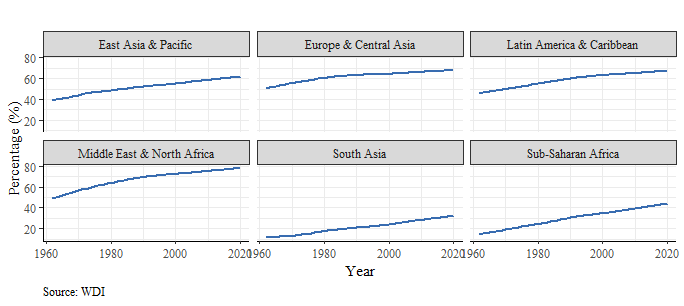
\includegraphics[scale = 0.8]{Graphics/urbanpopPercent.png}
    \caption{Average percent of people living in urban areas has been growing in regions around the world.}
    \label{fig:Urbanpopgrowth}
\end{figure}

Urbanization seems to trend according to the stage of development that nations are currently experiencing. Despite this, the fact remains that countries at every income class on average experience urban population growth rather than a decline (Figure 1). Slum populations on average as a proportion of urban populations, however, seem to be paradoxically decreasing (Figure 2). 

Although this is an aggregate trend and may not be the case in every country, it still raises questions about the factors that influence slum growth. Additionally, even though infrastructure spending seems to have on average experienced an upwards trend across regions relative to past decades (Figure 3), this trend doesn't seem to correlate well with the relative magnitudes of slum decline and some regions that don't experience any increase in infrastructure spending to match growing urban areas also witness a decline in slum proportions amongst urban populations.

\begin{figure}
    \centering
    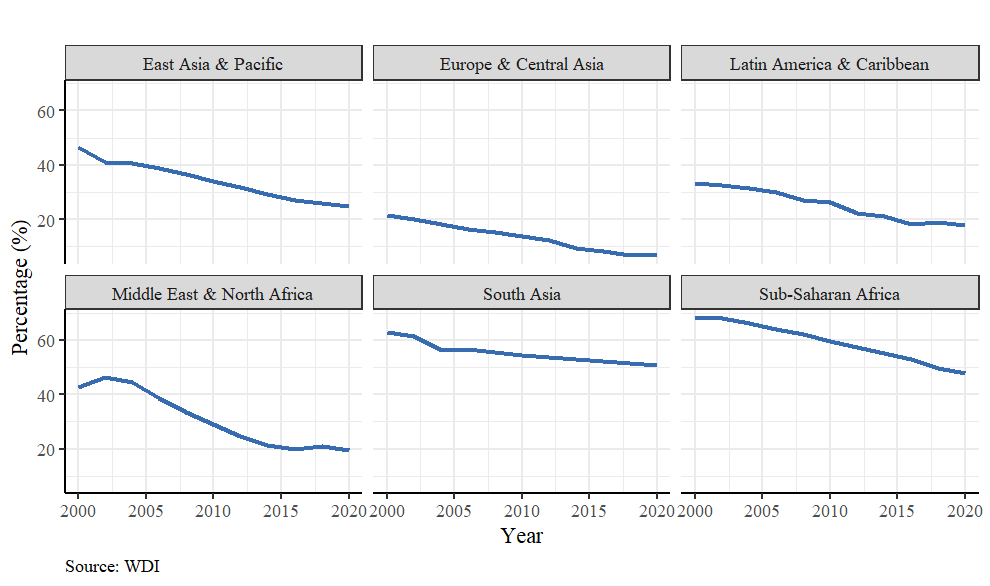
\includegraphics[scale = 0.8]{Graphics/Average Percent of urban households living in slums.png}
    \caption{Average percent of urban households living in slums has been on the decline in every global region.}
    \label{fig:SlumsTrend}
\end{figure}

\begin{figure}
    \centering
    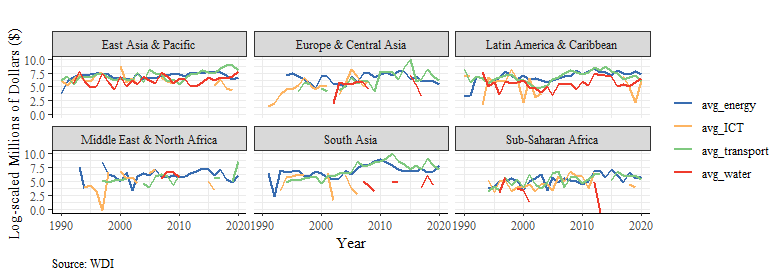
\includegraphics[height = 6cm]{Graphics/Average country-wide infrastructure spending per region.png}
    \caption{Average country-wide infrastructure spending per region}
    \label{fig:Infraspending}
\end{figure}

\begin{table}[ht]
\centering
\caption{Estimated total stocks of migration from, to, and within Africa\textsuperscript{{\cite{WBGBMD}}}}
\begin{tabular}{rlll}
  \hline \hline 
 & Africa to the rest of the world & Rest of the world to Africa & Within Africa\\ 
  \hline
1960 & 1 830 776 & 2 811 930 & 6 176 385 \\ 
1980 & 5 418 096 & 1 872 502 & 7 966 359  \\ 
2000 & 8 734 478 & 1 532 746 & 10 500 000  \\ 
   \hline
\end{tabular}
\end{table}

Despite their prevalence across the world, slums all have varying characteristics from region to region. This project, however, is focused on Sub-Saharan Africa since that is where most of the training data has been collected and is the region with the second-highest average proportion of urban populations living in slums. Urban movement in Africa is often miss-classified as a mass exodus from Africa to Western Nations, in fact, Africa has the lowest intercontinental out-migration rates of all world regions\textsuperscript{\cite{Teye}}. Although intercontinental migration, especially to Europe, has been on the rise in Africa itself, this has been primarily focused in North Africa and still pales relative to intracontinental migration within Africa itself which has also been increasing (Table 1). 


These migration patterns have a significant effect on the urban landscape in Africa. As is generally the case around the world, migration mobility in Africa has been seen to be linked to the wealth of a given country and its habitants. The wealthier an individual, the more facility they have to relocate, and relocate to further distances as well. This is why a significant proportion of urban movement lies within rural relocation to urban areas in search of greater opportunity. Teye explains that 
\begin{quoting}although a significant proportion of the rapid increase in urban population is caused by the high rate of natural increase in towns and re-classification of settlements into urban areas, migration accounts for a significant proportion urbanization in Africa. In some countries, rural-urban migration accounts for about 60\% of urban growth because rural-urban inequalities of development force people to move from rural areas to urban areas in search of jobs \textsuperscript{\cite{Teye}}.\end{quoting} 

The packing of poor groups of people into already overburdened urban areas due to the migratory movement of rural peoples into urban areas is what this paper studies. A significant amount of this paper will focus on Kenya, so it is important to take a cursory look at the migratory characteristics of Kenya as well. Figure 4 shows how urban population growth in Kenya has stayed fairly consistently positive over the past 30 years but slum proportions have been on the decline since 2000 (Figure 5). Infrastructure spending data in Kenya is sparse and is not enough to conclude some sort of trend.

\begin{figure}
    \centering
    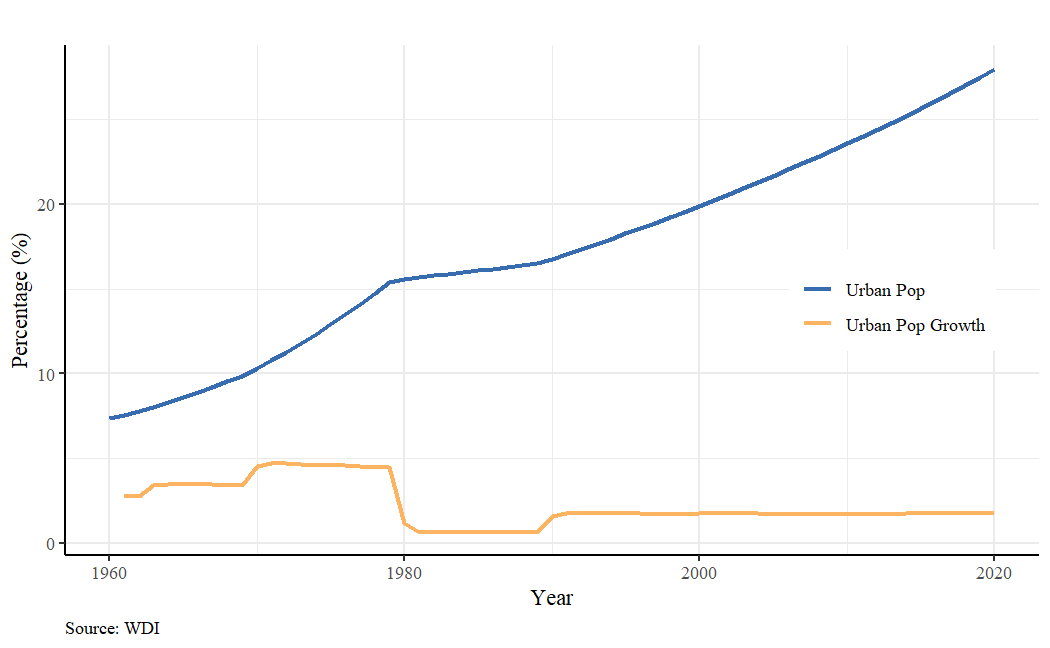
\includegraphics[scale = 0.65]{Graphics/Kenya Urban Population Percentage.png}    
    \caption{Urban population growth as a percentage of the total population of Kenya has stayed fairly consistent over the past 20 years.}
    \label{fig:KenyaUrban}
\end{figure}


\begin{figure}
    \centering
    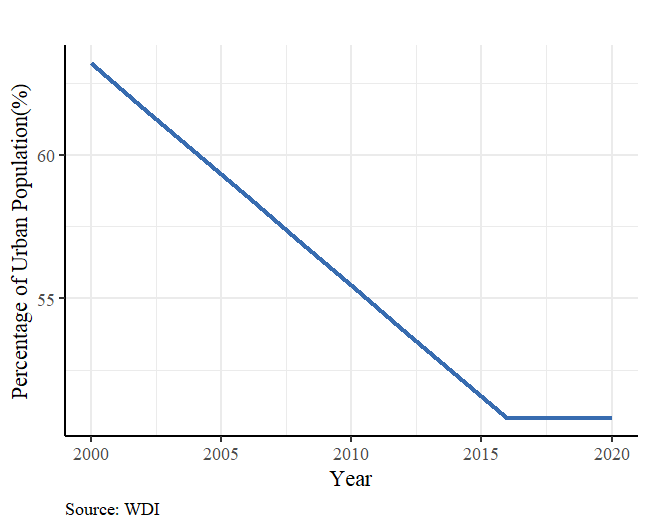
\includegraphics[scale = 0.8]{Graphics/Kenyan Urban Slums.png}
    \caption{Despite urban population growth, the slum proportion of urban populations has been on the decline}
    \label{fig:kenyanslums}
\end{figure}





\section{Relevance}

Although studying how slums comes to form is an interesting question in itself there are also a few reasons as to why we should be concerned with the formation and characterization of them beyond trying to find an explanation for the decline of slums despite urban populations increasing and unmatched spending on infrastructure. Even if one argues that some may prefer urban poverty to rural poverty there are several unique characteristics that slums pose that make them unique relative to the general case of lower income neighborhoods. Marx, Stoker, and Suri\textsuperscript{\cite{Marx}} explain that slums act as a poverty trap for the majority of their residents. They \begin{quoting}document how human capital threshold effects, investment inertia, and a policy trap may prevent slum dwellers from seizing economic opportunities offered by geographic proximity to the city.\end{quoting}

Slum mapping and prediction has been a relatively new area of interest. Some papers like Friesen, Rausch, Pelz, and Furnkranz\textsuperscript{\cite{wdislums}} try to analyze national indicators that are most correlated with urban slum populations using data from the World Bank and modeling methods such as Random Forest, JRIP (rule learning algorithm), and J48 (decision tree learner). Their data set, however, is not minute enough to make any meaningful claims. Using country-level effects to predict city-level indicators confounds many variables and can paint a wrong picture especially in countries in which the disparity between cities is large. On the other hand, new satellite imagery is allowing researchers to look at very small details that allow for a more micro level analysis. Image recognition software is being used to characterize photos with slums in order to have a more clear global pictures. Issues arise, however, in the accessibility and quantity of these high resolution satellite images.

Mapping and identification are critical to ensuring that potential future policy that targets slums is accessible to all the areas that need assistance. Marx, Stoker, and Suri\textsuperscript{\cite{Marx}} for example recommend a paradigm for policies to address the growth of slums but in order to begin any sort of action one must have proper documentation as a foundation for any concrete plans. In addition, although slums may be the symptom of greater forces at play rather than the disease itself, learning more about how they form and why an individual chooses to live in a slum is crucial to understanding what of those greater forces need attention.

Exploring slum growth contributes a lot to understanding key factors in development of cities and developing a micro-model on what pushes households to live in slums is a good step in learning about the formation of clusters of housing and neighborhoods. Discrete choice models for housing location is a well-established field\textsuperscript{\cite{Mackay}} but research on the specific slum related implications of these discrete choice models is relatively sparse and a new field. Studies are focused on data in the form of sample size limited household surveys from an individual city to bypass the issue of a lack of widely available data of the same sort\textsuperscript{\cite{Badmos},\cite{Celhay},\cite{Deeyah},\cite{Roy},\cite{Das}}.


The following work will be in two parts. The first to explore new avenues for mapping slums, particularly using a novel data set: the Defense Meteorological Satellite Program Operational Line Scanner (DMSP/OLS) Nighttime Light Image Timeseries from NOAA. The second part of this paper calibrates a basic discrete choice model that takes a micro economic glance at what factors drive households to live in slums. While we have a clue about the general correlation at a macro level of what motivates slum growth, identifying the systematic decision bias that is the threshold between choosing to live in a slum or not can help stimulate targeted policy action and give more insight as to what is driving down slums proportions despite an increase of urban populations.


\section{Data Processing}

The first portion of this paper uses a considerable amount of data and is primarily restricted by both computational power and availability of a database of slums. There are five primary categories that are listed below.
\begin{itemize}
    \item \textbf{Version 4 DMSP-OLS Nighttime Lights Time Series}\textsuperscript{\cite{lightdata}}
    
    This paper uses nighttime light images from 2000 to 2013 and to reduce computational expenditure whilst also improving model relevance since most of the training data set of identified slums is from African countries in 2013. Each pixel has a resolution of one square kilometer.
    
    \begin{figure}[ht]
        \centering
        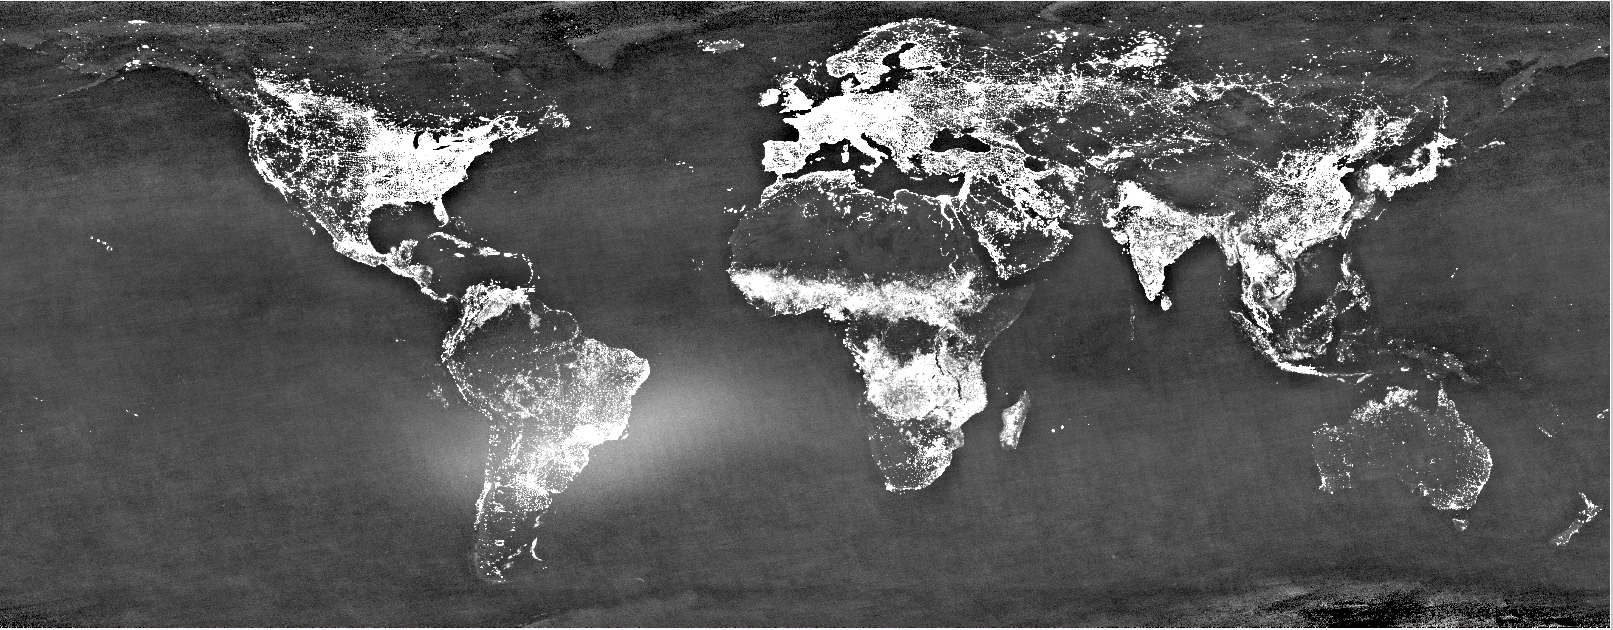
\includegraphics[scale = 0.3]{Graphics/F162008 avg lights pic.png}
        \caption{Averaged light values in 2008}
        \label{fig:F162008}
    \end{figure}
    
    This data set is the most novel out of all the other data sets in terms of usage in economics and it also requires special treatment on the processing end as well. These files are stored in a TIF format which are dense images which contain additional information at each pixel. In this case, each raw file download from NOAA contains an image of the world as below and must be processed first using spatial data processing software.    
    
    \item \textbf{World Pop Hub: Population Density Data}\textsuperscript{\cite{popdata}}
    
    The second data set that this paper is contingent on is population density. WorldPop.org is a very encompassing database that includes a granular count of population density with a resolution of 1 kilometer.
        
    \item \textbf{Slum Dwellers International}\textsuperscript{\cite{slumdata}}
    
    This data set acts as the training data set that includes already identified slums, their coordinates, and additional characteristics of the slum such as access to sanitation or public transportation. This data does not exist in a consolidated format and must be scraped from SDI.org. This information was collected by consulting locals to survey areas from 2013 to 2018 in cities that are widely considered by locals to be slums.

    \item \textbf{World Bank: World Development Indicators}\textsuperscript{\cite{wdislums}}

    When abstracting the mapping model to multiple countries, we would use a series of world bank indicators as controls - an extensive list of potential variables is included in Table 17 in the appendix - to distinguish countries from each other. Currently, I use the WDI indicators to calibrate the household choice model using data about slum population as a proportion of total urban population in countries.

    \item \textbf{Numbeo: Rent Characteristics of Countries}\textsuperscript{\cite{Numbeo}}

    This data set is also used to calibrate the household choice model. It consists of the aggregate results of surveys of various cities across countries which report on characteristics such as income and rent - among many others.
    
\end{itemize}

 Several decisions had to be made about the scope of the lights and population density data to consider since although data was plenty in these two areas, the slums data set was very limited. Making assumptions that the slums data set had profiled all the slums in a given country would drastically skew models as there might be many areas that are slums in real life and whose light and population density characteristics indicate to be so but are not captured in the slums data set. As such, lights and population density observations were taken from grid areas around cities we know were surveyed for slums. In the future, given a more precise slums data set, this paper can be much better tuned. 

Once all the data sets are individually processed, we still must merge them all by coordinate points. This introduces another set of assumptions. The first issue is the matching of coordinate points between the nighttime lights and population density data sets. There are several methods of conducting this matching process that vary in time complexity and accuracy. After conducting a time complexity and accuracy tradeoff analysis, this paper conducts the matching process by creating larger pixel grids, calculating the average population density of each larger grid space, and then assigning that new aggregate population density value to each of the smaller pixels within that larger grid unit. In addition, to classify coordinate points as slums or not, we have to do a similar process of first making a simplifying assumption that slums are spatially circular in nature and translate the square meter area into distance difference in geo-coordinates. This area to geo-coordinate translation also includes another simplifying assumption in that we disregard the curvature of the earth; this assumption, however, is minute and often taken as a given when working with physical areas as small as the ones in the slums data set. Once the radius of each slum is identified, calculating whether a geo-coordinate pair in the lights data set is regarded to be a slum is a simple issue of calculating if distance to the center of any of the documented slums is less than that given slum's radius.








\section{Exploratory Data Analysis}

\subsection{Compiled Dataset Summary Statistics}

Each data set has a number of unique qualities and there is quite a bit of data to cover in order to have a thorough discussion of each nuance. Regardless there are still quite a few trends to consider before engaging in the model making. Note that unless otherwise specified, data here is from 2013, which is what we will use to create the slum mapping models as the training slums data set is from 2013 as well.


% latex table generated in R 4.0.3 by xtable 1.8-4 package
% Thu Mar 16 02:08:41 2023
\begin{table}[ht]
\centering
\caption{2013 Kenya Cleaned Data Summary Statistics}
\begin{tabular}{rlrrrrrrr}
  \hline \hline
 & habitation & total\_count & avg\_light & avg\_pop & sd\_light & sd\_pop\\ 
  \hline
1 & Not a Slum & 28986 & 0.67 & 189.60 & 2.50 & 301.45\\ 
  2 & Slum & 22381 & 2.39 & 137.63 & 8.03 & 430.09\\ 
  3 & Uninhabited & 1650 & 8.89 & 0.00 & 16.68\\ 
   \hline 
\end{tabular}
\end{table}

Table 2 indicates that our data set is slightly imbalanced. The ratio of slum to no slum observations in the training data is approximately 1:1.295 which is relatively much better than proportions if we were to process data from the entire country which would imbalance the data set to a ratio of about 1:16. Next, to discern the mixed effects of lights and population density, I engineer two new categorical variables by discretizing the range of both of these values into five quantiles; each of which is represented by a bin number, where the lower the bin number, the lower the quantile value. 

\begin{figure}
    \centering
    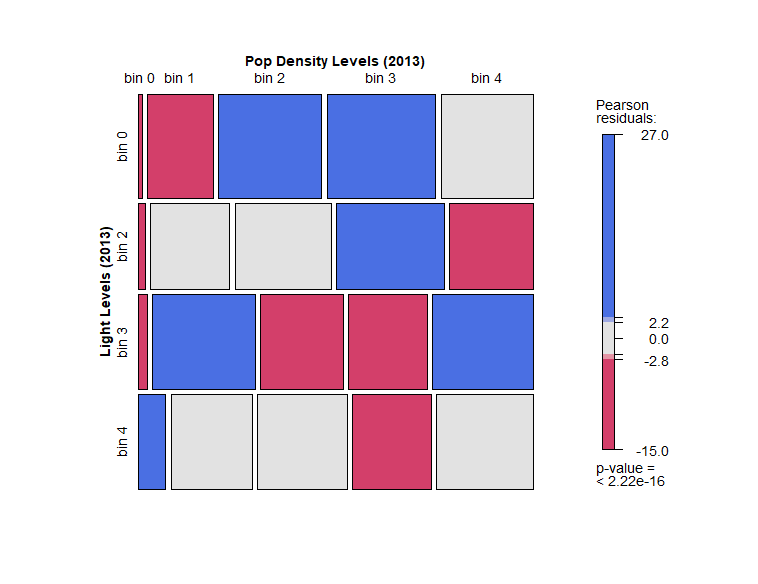
\includegraphics[scale = 0.36]{Graphics/Total Mosaic.png}
    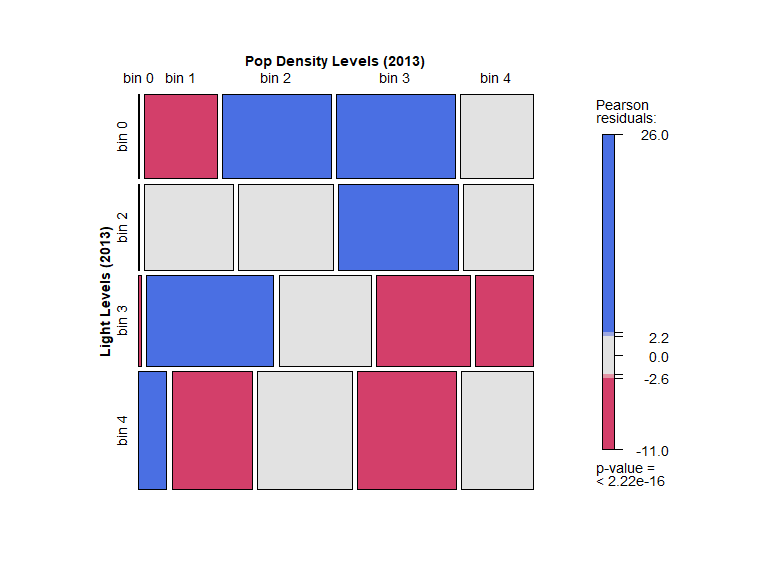
\includegraphics[scale = 0.36]{Graphics/Slum Mosaic.png}
    \caption{Distribution of lights and pop density values among slums is statistically biased}
    \label{fig:mosaic1}
\end{figure}

Before we delve into any of the model building, Figure 7 is a quick check for homogeneity of these categorical variables amongst both positive slum observations and the entire dataset. We can see some promising initial evidence that the distribution of slums does have a statistical bias towards low light levels and high population density, although there is also a few clusters at high light levels and low population density. At a qualitative level, the marginal distributions of the continuous population density and light values conditioned on a location being a slum or not seem to be about similar. But the sheer magnitude of the sample size reveals a different story when looking at statistical tests and show that there are indeed statistically significant differences in the means of the distribution and between the distribution as a whole at a 95\% confidence level.

\begin{table}[ht]
\centering
\caption{Distribution Tests}
\begin{tabular}{rlrrr}
  \hline \hline
 & Test & p-value & df & t-score \\ 
  \hline
1 & Two-sample Kolmogorov  & $<2.2e-16$ &  &   \\
 & Smirnov test & & &  \\
 \hline
  2 & Welch Two & $< 2.2e-16$ & 25752 & 30.849 \\
   & Sample T-test & & & \\
   \hline
\end{tabular}
\end{table}


\begin{figure}
    \centering
    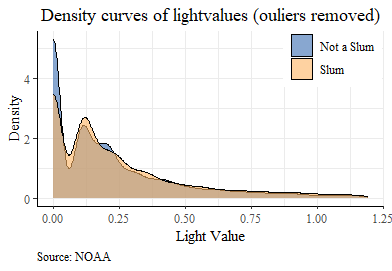
\includegraphics[scale = 0.7]{Graphics/Light Value density curve.png}
    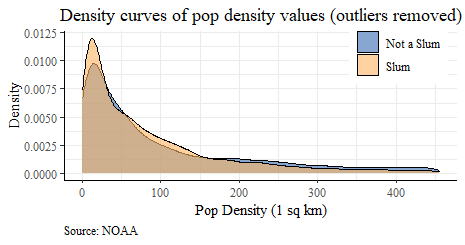
\includegraphics[scale = 0.75]{Graphics/Pop Density density curve.png}
    \caption{Distribution of lights and population density is heavily skewed towards smaller values}
    \label{fig:densitycurves}
\end{figure}

In the context of modeling, however, I discretize the continuous domain of light and population density values to capture the hypothesized non-linear effects of the interaction between population density and nighttime lights. For the basic model I break the light values into five quantiles and assign each observation's light value and population density value into a "bin" corresponding to their quantile. Figure 9 shows the distribution when we discretize the two features into ten bins: although population density seems to be approximately normally distributed with a high variance, the lights bins do not seem to be as well behaved as most light values tend to be very low and the bottom three quantiles are all the same.

\begin{figure}
    \centering
    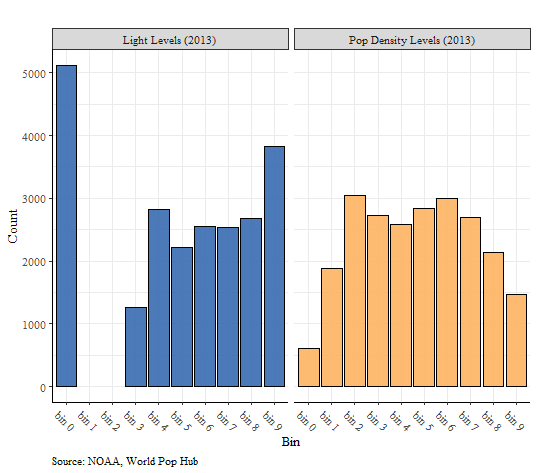
\includegraphics[scale = 0.7]{Graphics/10BinsBar.png}
    \caption{Caption}
    \label{fig:2013discretizeddistr}
\end{figure}

The benefit of increasing the number of bins is that we can capture a bit more non-linearity the models than with lower bins, but increasing the number of bins also has an added effect of potentially over-fitting and reducing the interpretability of the model: it no longer becomes a question of "low" and "high" light values but more so model effects contingent on individual bins and little insight into trends in the behavior of the data. It is important to note that the range of values, especially on the highest bin, may vary a lot due to outliers but cropping outliers can often times remove very key pieces of information since outliers in the context of this data often refers to city centers or very densely populated areas of a city which we have hypothesized may be home to slums.

\begin{figure}
    \centering
    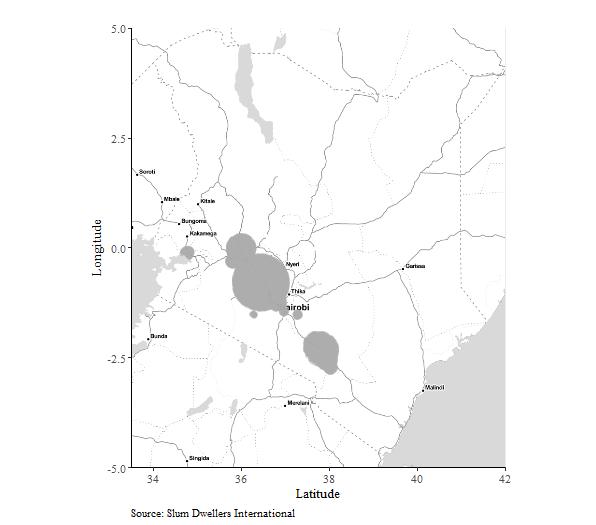
\includegraphics[scale = 0.6]{Graphics/Approximated Spatial Distribution of Slums in Kenya.png}
    \caption{Approximated Spatial Distribution of Slums in Kenya}
    \label{fig:slumMap}
\end{figure}

Finally, the data this paper works with is primarily spatial in nature: each observation is a latitude, longitude geo-coordinate pair. From an initial glance, we can clearly see assumptions about the shape of slums at play. Future iterations of the paper will embellish upon the slums data set and define more precise slum boundaries to better capture potential light and population density effects.




\subsection{Growth Accounting}

It is important to note that in this paper, we treat light values and population density as a potential indicator of slums rather than there being some causal relationship. The main drivers of slum formation is likely the state of the economy and key characteristics such as the ratio between wages and rents which may in turn be connected to lights. We explore these macro relationships as well to gain more insight into any indirect effects. To begin, as the title of this subsection entails, Figure 11 shows the solow macro model growth dynamics for Kenya. Note that we have not detrended GDP and as such we see that the main reason GDP growth is not as high as it should be is due to low capital.

\begin{figure}
    \centering
    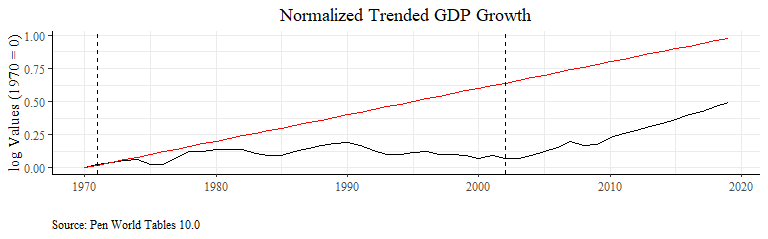
\includegraphics[scale = 0.7]{Graphics/Normalized Trended GDP Growth.png}
    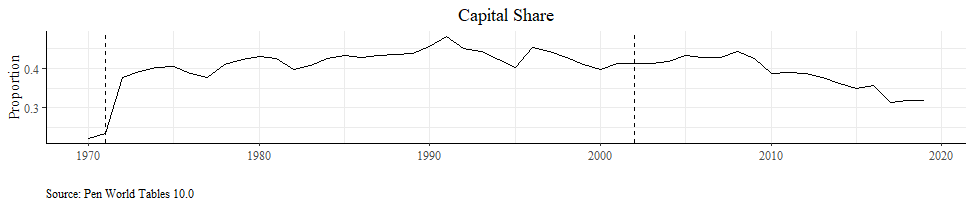
\includegraphics[scale = 0.52]{Graphics/Capital Share.png}
    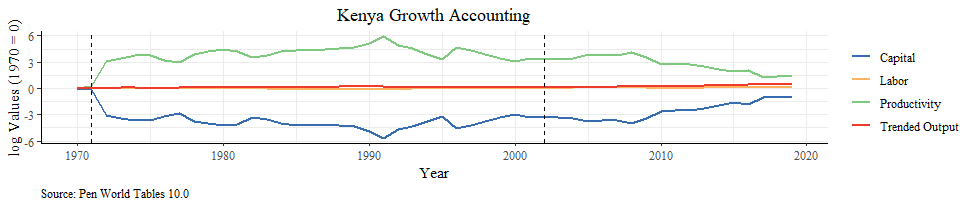
\includegraphics[scale = 0.52]{Graphics/Kenya Growth Accounting.png}
    \caption{Cobb Douglas Growth Accounting (Variable Alpha) - Kenya}
    \label{fig:KenyaGrowthAccounting}
\end{figure}

To further investigate, figure 12 shows both how aggregate average lights per square kilometer and population density per square kilometer in Kenya has fared from 2000 to 2013. As further insight into relationships between lights, population density and how a potential indirect relationship may be, the second graphic below displays the simple linear regressions of both lights and year on GDP, and GDP and year on lights. In both cases, the impact of light on GDP and GDP on light have statistically significant positive coefficients which speaks to potential confounders in terms of establishing a causal relationship between population density and light. Since we are initially only trying to estimate an indicative relationship to use as a tool to map, this confounder in the causal relationship is good because it establishes a link between slums and lights.

\begin{figure}
    \centering
    \begin{minipage}{0.45\textwidth}
    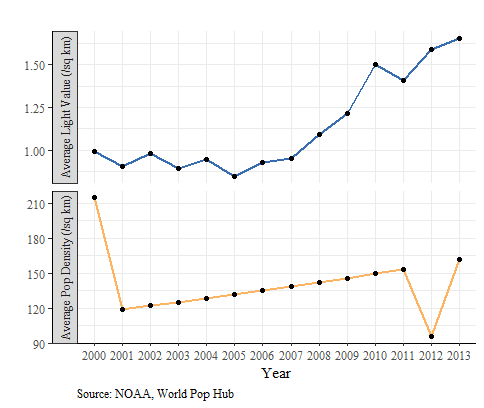
\includegraphics[scale = 0.55]{Graphics/Average lights and population density over time.png}
    \caption{Kenya, Average lights and population density over time}
    \end{minipage}
    \begin{minipage}{0.45\textwidth}
    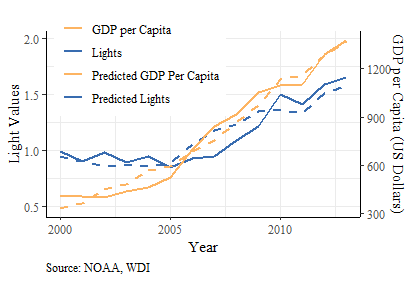
\includegraphics[scale = 0.8]{Graphics/Kenya, Average lights and GDP per Capita over time.png}
    \caption{Kenya, Average lights and GDP per Capita over time}
    \label{fig:lightpoptime}
    \end{minipage}
\end{figure}



% latex table generated in R 4.0.3 by xtable 1.8-4 package
% Mon Mar 20 00:52:26 2023
\begin{table}[ht]
\centering
\caption{Correlation Plot (GDP is per capita)}
\begin{tabular}{r|rrrrr}
  \hline\hline
 & Year & GDP & Pop Density & Lights & Detrended GDP \\ 
  \hline
Year & 1.00 & 0.97 & -0.12 & 0.85 & 0.98 \\ 
  GDP & 0.97 & 1.00 & -0.01 & 0.91 & 0.99 \\ 
  Pop Density & -0.12 & -0.01 & 1.00 & 0.05 & -0.02 \\ 
  Lights& 0.85 & 0.91 & 0.05 & 1.00 & 0.85 \\ 
  Detrended GDP & 0.98 & 0.99 & -0.02 & 0.85 & 1.00 \\ 
   \hline 
\end{tabular}
\end{table}


\section{Modeling}

\subsection{Slum Mapping}

The primary purpose of the mapping models is twofold: to identify if there is some level of relationship between nighttime light values, population density, and the location of slums, and second to create a model that is able to provide data on slum locations to use later in the calibration of the household decision model. Due to restrictions on available computational power, this paper uses data only from surveyed slums in Kenya: as such, there is no need for any country level control variables. One key factor to remember is that since the following models only train on data from Kenya, any model interpretation will reveal only characteristics about Kenyan slums or slums in countries and cities that are very similar to Kenya.

\subsubsection{Model 1: Vanilla Logistic Regression}
We begin with a bare-bones logistic regression model. To discern the mixed effects of lights and population density, remember that we discretize the range of both of these values into five quantiles. We then interact these two new engineered categorical variables in the model. The initial logistic regression model is shown in Table 5.

% Table created by stargazer v.5.2.2 by Marek Hlavac, Harvard University. E-mail: hlavac at fas.harvard.edu
% Date and time: Sun, Apr 02, 2023 - 12:08:09 PM
\begin{table}[!htbp] \centering 
  \caption{Small extract from vanilla logit table} 
  \label{Vanilla Regression Table} 
\begin{tabular}{@{\extracolsep{5pt}}lc} 
\\[-1.8ex]\hline 
\hline \\[-1.8ex] 
 & \multicolumn{1}{c}{\textit{Dependent variable:}} \\ 
\cline{2-2} 
\\[-1.8ex] & slum \\ 
\hline \\[-1.8ex] 
  Light Bin 4 and Pop Density Bin 0 & 2.611$^{***}$ \\ 
  & (0.404) \\ 
  & \\ 
 Light Bin 0 and Pop Density Bin 4 & 1.430$^{***}$ \\ 
  & (0.398) \\ 
  & \\ 
 Light Bin 4 and Pop Density Bin 1 & $-$2.050$^{***}$ \\ 
  & (0.410) \\ 
  & \\
 Light Bin 4 and Pop Density Bin 4 & $-$2.085$^{***}$ \\ 
  & (0.409) \\ 
  & \\ 
\hline \\[-1.8ex] 
Observations & 31,810 \\ 
Log Likelihood & $-$20,911.600 \\ 
Akaike Inf. Crit. & 41,863.200 \\ 
\hline 
\hline \\[-1.8ex] 
\textit{Note:}  & \multicolumn{1}{r}{$^{*}$p$<$0.1; $^{**}$p$<$0.05; $^{***}$p$<$0.01} \\ 
\end{tabular} 
\end{table} 

These results bode well for the initial hypothesis that slums tend to appear in areas with low light level values, but also seems to indicate that in general, low light level values are a good indicator of slums regardless of population density, and the biggest factor that contributes towards areas not being considered as slums is the highest bin of light values. Results for population density are a bit more inconclusive in terms of determining a general trend. Ultimately, the biggest takeaway is that low light level values drive the biggest increase in the log odds of a specific geo-coordinate observation being considered a slum and the highest light level values are the biggest drivers of decreasing the log odds of a specific geo-coordinate observation being considered a slum.

Although there seems to be promising statistical significance results it is important to assess the predictive ability of this model as well. Logistic regression prediction often considers a prediction probability threshold of 0.5, this is, however, one hyperparameter than can be tuned and optimized for the sake of arriving at a better predictive model. 

%latex table generated in R 4.0.3 by xtable 1.8-4 package
% Tue Feb 07 21:15:33 2023
\begin{table}[ht]
\centering
\caption{Logit Model 1 Validation error metrics}
\begin{tabular}{llll}
  \hline \hline 
  Error Metric &  Slum Predictions &  Slum Observations  & Error Rate \\ 
  \hline
Total data set & 2696 & 10604 & 0.4048472 \\ 
Positive Slum Observations & 1525 & 4647 & 0.6718313\\
   \hline
\end{tabular}
\end{table}

After conducting a grid search through potential threshold values we see that we can drastically increase slum predictive accuracy while only sacrificing a little accuracy in the context of the entire data set. Finally, Figure 15 provides a spatial view of how the model seems to be performing using a prediction threshold of 0.4.

\begin{figure}
    \centering
    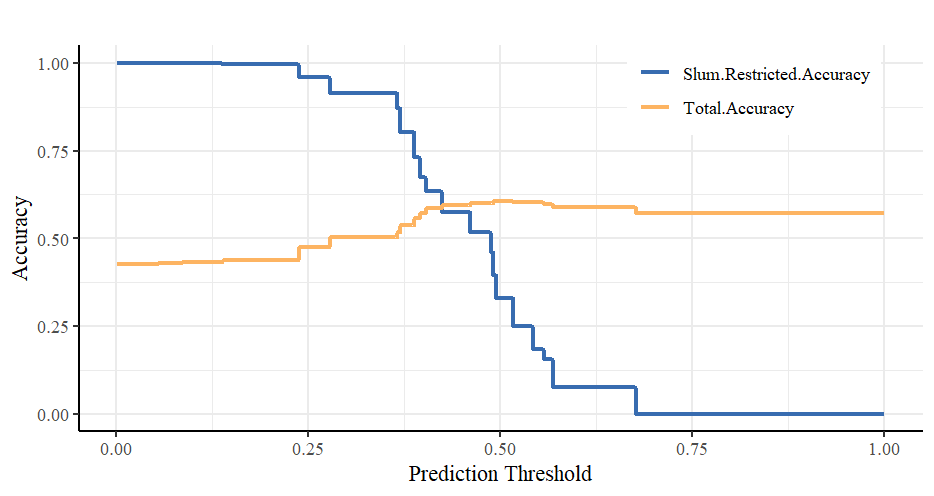
\includegraphics[scale = 0.8]{Graphics/Vanilla Slums and Total Dataset Accuracy Tradeoff.png}
    \caption{Vanilla Logit Slums and Total data set Accuracy Tradeoff}
    \label{fig:vanillaModelTradeoff}
\end{figure}

\begin{figure}
    \centering
    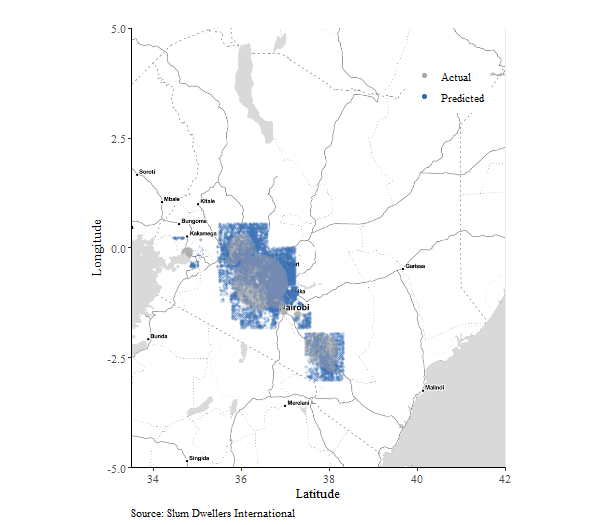
\includegraphics[scale = 0.7]{Graphics/Vanilla Predicted Spatial Distribution of Slums in Kenya.png}
    \caption{Vanilla Logit Model Predicted Spatial Distribution of Slums in Kenya}
    \label{fig:vanillaPredict}
\end{figure}

\subsubsection{Model 2: Logit with Increased Bins}

Having a data set with only five bins creates a lot of potential for categorizing values that are drastically different from each other into the as the same bin value. One way to address this issue is to increase the number of bins. 

\begin{figure}
    \centering
    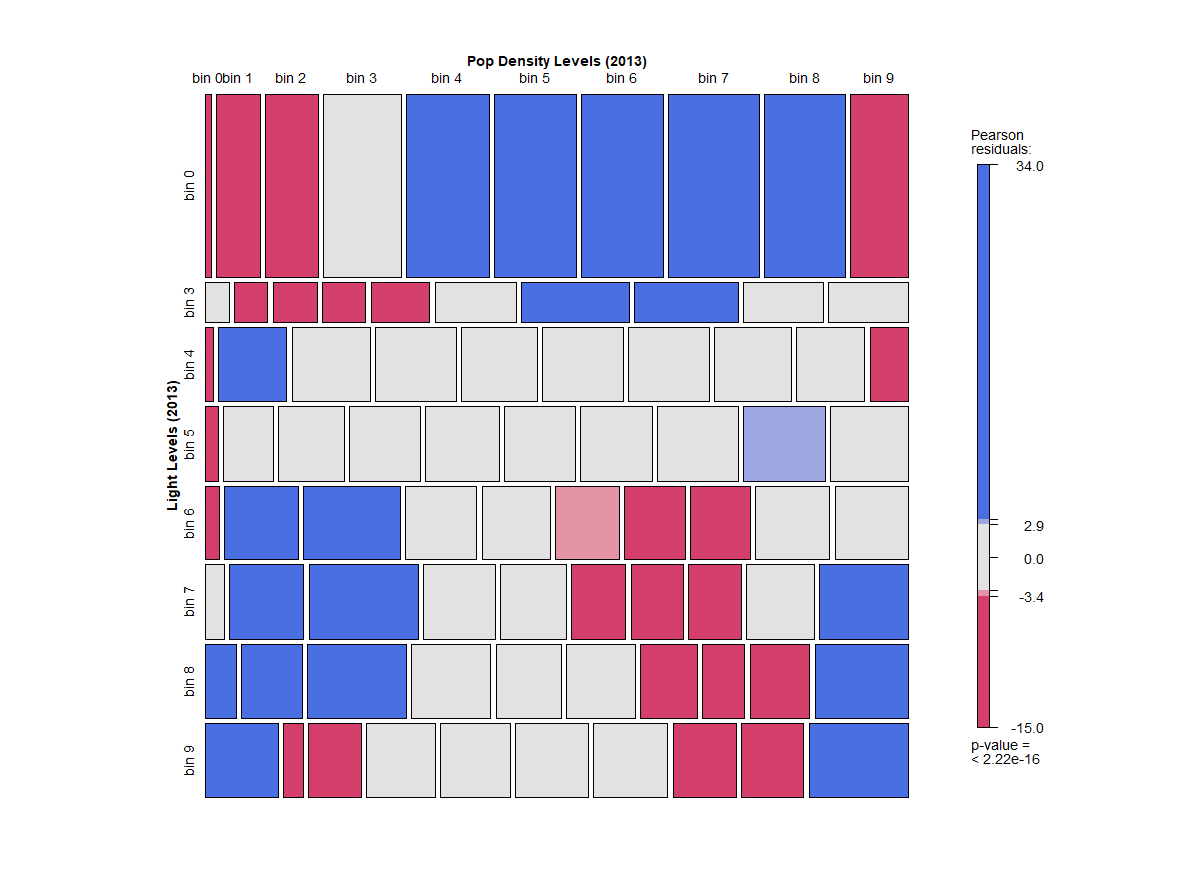
\includegraphics[scale = 0.225]{Graphics/Total Mosaic Bins.png}
    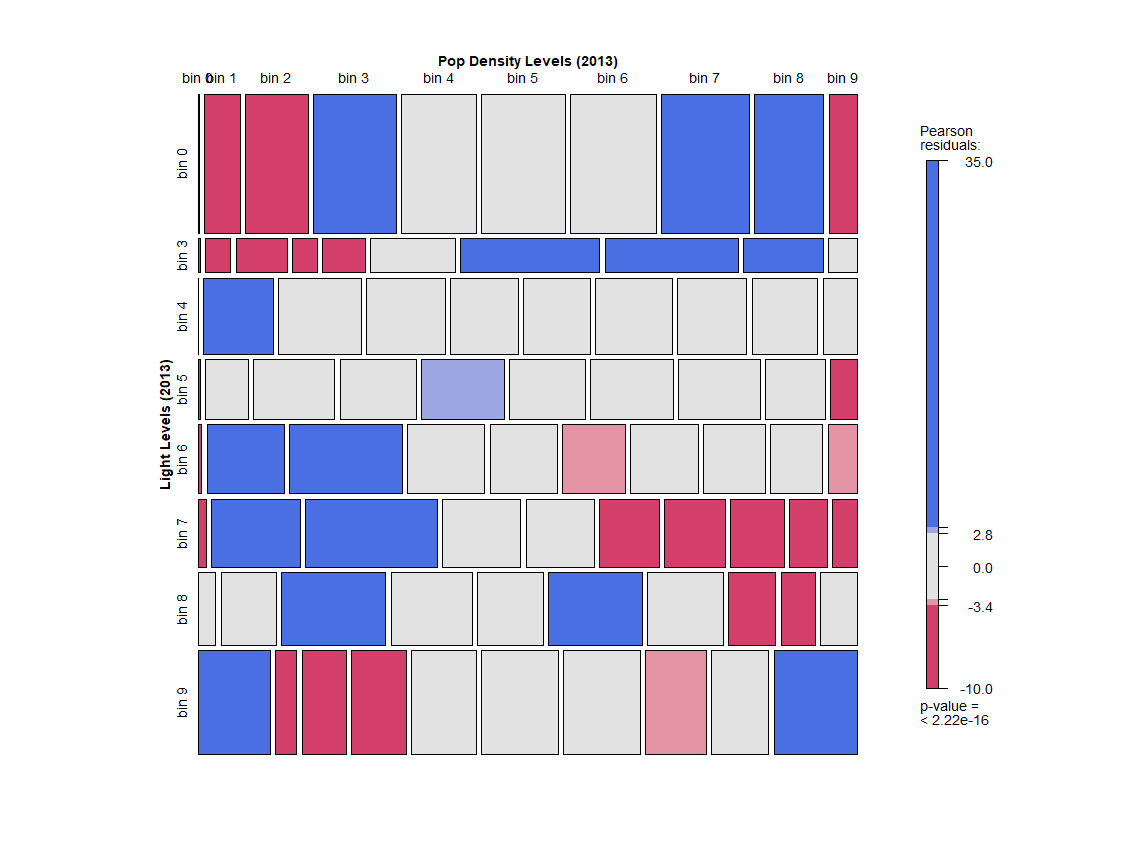
\includegraphics[scale = 0.23]{Graphics/Slum Mosaic Bins.png}
    \caption{Mosaic plot with 10 bins shows similar levels of heterogeneity in distribution of lights and population density}
    \label{fig:binsMosaic}
\end{figure}

Again, the mosaic plots indicate a similar story as with the data with just five bins. There is, however, additional nuance with the extreme high light and population density values.

% Table created by stargazer v.5.2.2 by Marek Hlavac, Harvard University. E-mail: hlavac at fas.harvard.edu
% Date and time: Sun, Apr 02, 2023 - 12:11:57 PM
\begin{table}[!htbp] \centering 
  \caption{Small extract of bins logit regression table} 
  \label{Bins Regression Table} 
\begin{tabular}{@{\extracolsep{5pt}}lc} 
\\[-1.8ex]\hline 
\hline \\[-1.8ex] 
 & \multicolumn{1}{c}{\textit{Dependent variable:}} \\ 
\cline{2-2} 
\\[-1.8ex] & slum \\ 
\hline \\[-1.8ex] 
Light Bin 0 and Pop Density Bin 8 & 1.632$^{***}$ \\ 
  & (0.400) \\ 
  & \\ 
 Light Bin 9 and Pop Density Bin 2 & $-$2.616$^{***}$ \\ 
  & (0.435) \\ 
  & \\ 
 Light Bin 4 and Pop Density Bin 9 & 1.864$^{**}$ \\ 
  & (0.842) \\ 
  & \\ 
 Light Bin 9 and Pop Density Bin 9 & $-$1.386$^{***}$ \\ 
  & (0.430) \\ 
  & \\ 
\hline \\[-1.8ex] 
Observations & 31,810 \\ 
Log Likelihood & $-$20,442.560 \\ 
Akaike Inf. Crit. & 41,045.130 \\ 
\hline 
\hline \\[-1.8ex] 
\textit{Note:}  & \multicolumn{1}{r}{$^{*}$p$<$0.1; $^{**}$p$<$0.05; $^{***}$p$<$0.01} \\ 
\end{tabular} 
\end{table} 


Once more, the regression results relate a remarkably similar story as with the logistic regression model with only five bins. As a whole, the predictive capabilities of this model seem to be a bit worse than that of the normal logistic regression with 5 bins with respect to general error metrics at a predictive threshold of 0.5. Again after conducting a gridsearch through potential threshold values, however, we see that we can drastically increase slum predictive accuracy while only sacrificing a little accuracy in the context of the entire data set a bit more than the previous regression model with only five bins. Finally, Figure 18 provides a spatial view of how the model seems to be performing using a prediction threshold of 0.4 and shows how it is able to mark one more slum area near Kakamega which the previous model was not able to do.

\begin{figure}
    \centering
    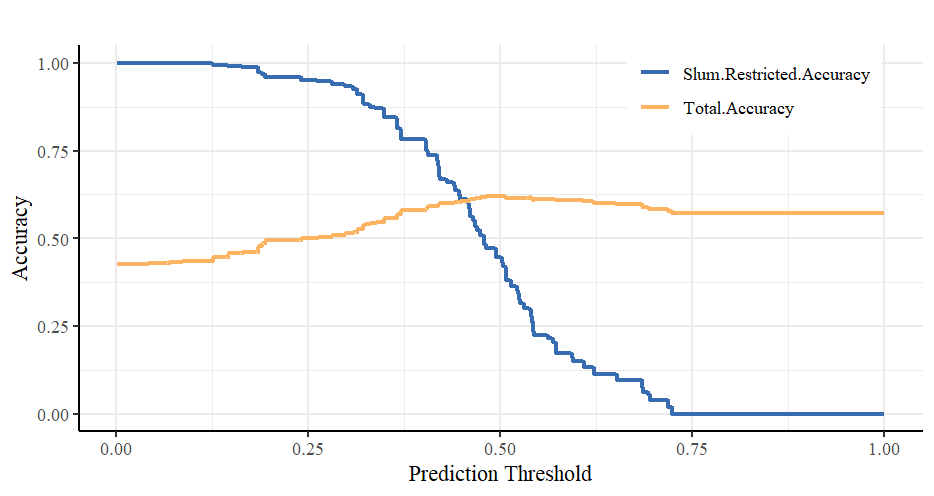
\includegraphics[scale = 0.8]{Graphics/Bins Slums and Total Dataset Accuracy Tradeoff.png}
    \caption{Bins Logit Model Slums and Total data set Accuracy Tradeoff}
    \label{fig:binsModelTradeoff}
\end{figure}



\begin{figure}
    \centering
    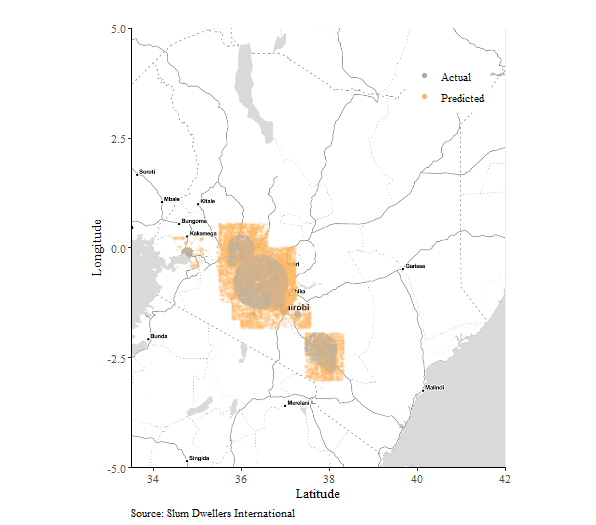
\includegraphics[scale = 0.6]{Graphics/Bins Predicted Spatial Distribution of Slums in Kenya.png}
    \caption{Bins Logit Model Predicted Spatial Distribution of Slums in Kenya}
    \label{fig:binsPredict}
\end{figure}

%latex table generated in R 4.0.3 by xtable 1.8-4 package
% Tue Feb 07 21:15:33 2023
\begin{table}[ht]
\centering
\caption{Logit Model 2 Validation error metrics}
\begin{tabular}{llll}
  \hline \hline
  Error Metric &  Slum Predictions &  Slum Observations  & Error Rate \\ 
  \hline
Total data set & 2759 & 10604 & 0.3904187 \\ 
Positive Slum Observations & 1651 & 4638 & 0.6474482\\
   \hline
\end{tabular}
\end{table}
\subsubsection{Model 3: Weighted Logit}



Within the current data set, the distribution of slums and no slum data points is relatively balanced. This property may not, however, extrapolate to other cities or data sets that undergo less pre-processing to consider only data from select cities and rural areas. Models trained on this data are drastically unbalanced and favor negative predictions resulting in models with exceptionally low overall accuracy but near a near 100\% false positive rate. As such, to better adapt to future applications of this research onto different data sets we also consider a weighted logistic regression that is biased towards slums. In the case of this initial model, we double weight slums relative to no-slum observations. The regression results are in Table 9 and indicate a similar story to the other models as well. Locations that have low light levels and high population density increase the likelihood of that location being a slum but more so high light level values decrease the likelihood of a location being a slum regardless of the population density level of that area.

%latex table generated in R 4.0.3 by xtable 1.8-4 package
% Tue Feb 07 21:15:33 2023
\begin{table}[ht]
\centering
\caption{Logit Model 3 Validation error metrics}
\begin{tabular}{llll}
  \hline \hline
  Error Metric &  Slum Predictions &  Slum Observations  & Error Rate \\ 
  \hline
Total data set & 9055 & 10604 & 0.3564527 \\ 
Positive Slum Observations & 2997 & 4657 & 0.35645265\\
   \hline
\end{tabular}
\end{table}

% Table created by stargazer v.5.2.2 by Marek Hlavac, Harvard University. E-mail: hlavac at fas.harvard.edu
% Date and time: Sun, Apr 02, 2023 - 2:47:57 PM
\begin{table}[!htbp] \centering 
  \caption{Small extract of weighted logit regression table} 
  \label{} 
\begin{tabular}{@{\extracolsep{5pt}}lc} 
\\[-1.8ex]\hline 
\hline \\[-1.8ex] 
 & \multicolumn{1}{c}{\textit{Dependent variable:}} \\ 
\cline{2-2} 
\\[-1.8ex] & slum \\ 
\hline \\[-1.8ex]
 Light Bin 0 and Pop Density Bin 4 & 1.430$^{***}$ \\ 
  & (0.293) \\ 
  & \\ 
 Light Bin 4 and Pop Density Bin 1 & $-$2.050$^{***}$ \\ 
  & (0.306) \\ 
  & \\ 
 Light Bin 2 and Pop Density Bin 4 & 0.887$^{**}$ \\ 
  & (0.397) \\ 
  & \\ 
 Light Bin 4 and Pop Density Bin 4 & $-$2.085$^{***}$ \\ 
  & (0.305) \\ 
  & \\
\hline \\[-1.8ex] 
Observations & 31,810 \\ 
Log Likelihood & $-$29,378.180 \\ 
Akaike Inf. Crit. & 58,796.350 \\ 
\hline 
\hline \\[-1.8ex] 
\textit{Note:}  & \multicolumn{1}{r}{$^{*}$p$<$0.1; $^{**}$p$<$0.05; $^{***}$p$<$0.01} \\ 
\end{tabular} 
\end{table} 


\begin{figure}
    \centering
    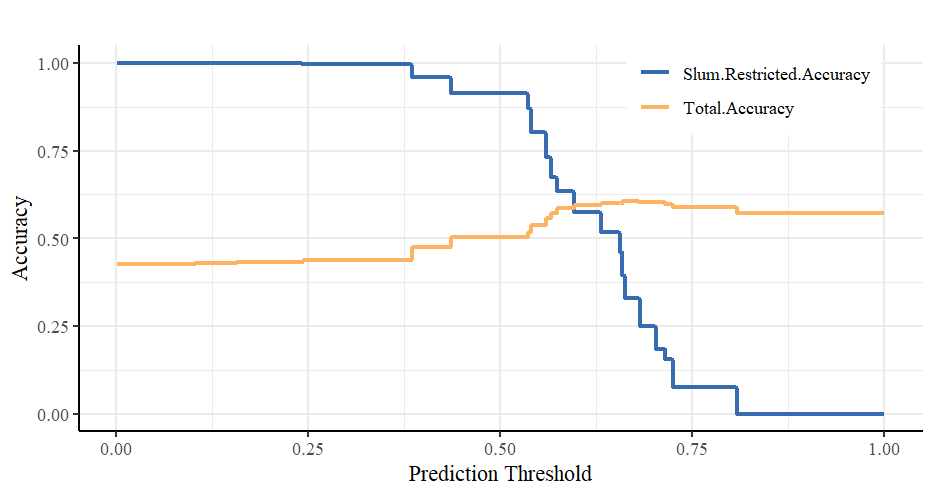
\includegraphics[scale = 0.8]{Graphics/Weighted Slums and Total Dataset Accuracy Tradeoff.png}
    \caption{Weighted Model Slums and Total data set Accuracy Tradeoff}
    \label{fig:weightedModelTradeoff}
\end{figure}



\begin{figure}
    \centering
    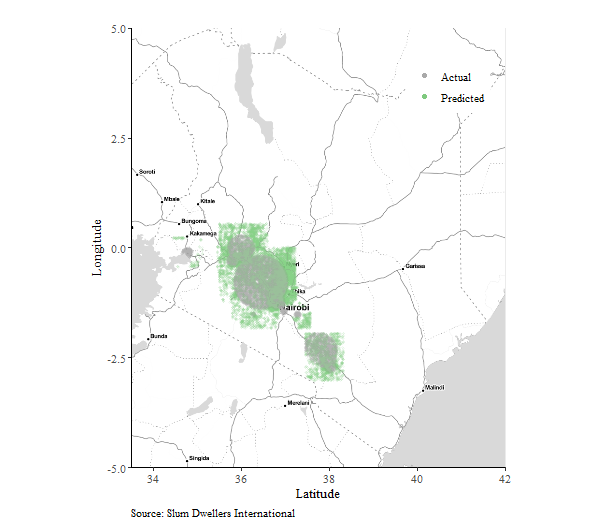
\includegraphics[scale = 0.6]{Graphics/Weighted Predicted Spatial Distribution of Slums in Kenya.png}
    \caption{Weighted Logit Model Predicted Spatial Distribution of Slums in Kenya}
    \label{fig:weightedPredict}
\end{figure}
The error metrics, created at a 0.6 probability prediction threshold level, also seem to fare a bit better for the weighted model. As a whole, the weighted model seems to perform a lot better than the previous two models. There are a lot fewer false positive slum attributions and the overall error metrics also seem to fair a decent proportion better; the qualitative predictive map shows that there are a fewer false positives as well.

\subsubsection{Model 4: Random Forest}

To conclude the predictive modeling portion of the paper we will test a random forest model. This model is a bit different in that it is a blackbox model and so causal interpretability will be much lower than in the previous models; we will not be able to conclude which conditions exactly cause a positive or negative slum observation. Regardless it is a good exercise in identifying if this type of model would have any better predictive power. Similar to the discussion in the previous modeling section, in further applications, data sets may not be as balanced between positive and negative slum observations and decision tree-based classification algorithms tend to be good at addressing these unbalanced data sets.

\begin{figure}
    \centering
    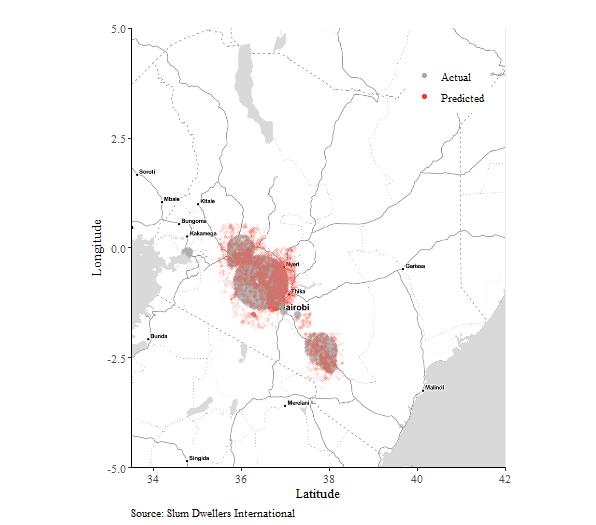
\includegraphics[scale = 0.6]{Graphics/RF Predicted Spatial Distribution of Slums in Kenya.png}
    \caption{Random Forest Model Predicted Spatial Distribution of Slums in Kenya}
    \label{fig:rfPredict}
\end{figure}

\begin{table}[ht]
\centering
\caption{Random Forest variable importance}
\begin{tabular}{ll}
  \hline \hline
  Variable &  Mean Decrease Gini\\ 
  \hline
Nighttime Lights & 5140.58 \\ 
Population Density & 6095.28\\
   \hline
\end{tabular}
\end{table}


In aggregate, the Random Forest model has better error metrics than the first two models but performs worse than the weighted logistic regression. We can see in the map visualization that it doesn't seem to make as many positive slum predictions relatively to the other model and as such its false positive rate is significantly lower than any of the other models. Interestingly enough, the variable importance plots indicate that contrary to the qualitative conclusions of the logit models, population density seems to be more important in making a slum prediction in this Random Forest model.

\begin{table}[ht]
\centering
\caption{Random Forest Model Validation error metrics}
\begin{tabular}{llll}
  \hline \hline
  Error Metric &  Slum Predictions &  Slum Observations  & Error Rate \\ 
  \hline
Total data set & 3399 & 10604 & 0.3564527 \\ 
Positive Slum Observations & 2085 & 4530 & 0.539735099\\
   \hline
\end{tabular}
\end{table}




\subsubsection{Final Comparative Analysis}

Ultimately, each model constructed serves a different purpose contingent on properties of the underlying training data set. Table 13 reports on one yet undiscussed comparative metric: area under curve (AUC) values for the receiver operating characteristic (ROC) curve of each model which provides an aggregate measure of performance across all possible classification thresholds. Note that this is a metric that doesn't capture the best level of error metrics for a model but rather some measure of overall robustness over various classification thresholds. In general, for the AUC values and other error metrics as well we see that there are some definitive differences, and this is especially also made clear in the visual depiction of the predictions that each of the models make. Regardless, the magnitude of the differences in metrics in each of the models speak to the level of robustness of the problem declaration: the ability to be able to map slums based on nighttime light and population density data. Better tuned training data and drawing training data from a larger set of countries may produce a much more accurate model.

\begin{table}[ht]
\centering
\caption{AUC values for ROC curve of each model}
\begin{tabular}{ll}
  \hline \hline
  Model &  AUC\\ 
  \hline
Vanilla Logit & 0.6272 \\ 
Bins Logit & 0.6581\\
Weighted Logit & 0.6272\\
Random Forest & 0.6675385\\
   \hline
\end{tabular}
\end{table}

\subsection{Household Spatial Choice Models}

As of yet, this paper has been a statistics question regarding how one can build a model to identify where slums are located based on nighttime light and population density data. The next parts of this paper will build a decision model for households that face the choice between living in different areas. There are two ways to model the decision-making process that households face. We can determine which to use in the future based on the availability of data since data availability is the one of, if not the biggest issue when working with developing countries. Finding very detailed spatial information for each county let alone each square kilometer is a herculean task. As such, the following sections will detail two model building processes; the first is a simplistic set up that I  will calibrate using not so perfect data and some assumptions, the second model will give a more detailed look at an idealistic model setup for exploring the questions of location choice but will not undergo any calibration. In both cases, however, I will specify an ideal data set for the calibratoin of each model. You can also refer to the appendix for ongoing work concerning simulating the growth of cities given households with utility functions similar to the one specified in the second more detailed choice model.

\subsubsection{Binary Choice Model}

The first, more simplistic setup is a two-choice model where households can choose whether or not they want to live in a slum or in an area in the city that is not a slum. To formalize, consider the problem setup; a household must choose whether to live in a slum $S_{slum}$ or in the main non-slum city $S_{city}$. The household's rent $r$ and wage $w$ is determined by where they live, and we can define the utility of living in either location as \begin{align}\begin{cases}
    U_{city} &= w_{city} - r_{city} + \epsilon_{city}\\
    U_{slum} &= w_{slum} - r_{slum} + \epsilon_{slum}
    \end{cases}\end{align}
    It would then follow that we are trying to identify the probability \begin{align}\begin{split}
        p(S_{slum}) &= p(U_{slum} > U_{city})\\
                    &= p(w_{slum} - r_{slum} + \epsilon_{slum} > w_{city} - r_{city} + \epsilon_{city})\\
                    &= p(w_{slum} - w_{city} + r_{city} - r_{slum} > \epsilon_{city} - \epsilon_{slum})\\
                    &= \int_{\epsilon}I(w_{slum} - w_{city} + r_{city} - r_{slum} > \epsilon_{city} - \epsilon_{slum}) f(\epsilon)\,d\epsilon
    \end{split}\end{align} 
    For binary choice models, one commonly used tool is a logistic regression which assumes that each error term is independently identically distributed and assumes the density and cumulative distributive functions are as follows \begin{align}
        \begin{split}
        f(\epsilon) &= \exp(-\epsilon)\cdot \exp(-\exp(\epsilon)),\\
        F(\epsilon) &= \exp(-\exp(\epsilon)),\\
        F(\epsilon_{city} - \epsilon_{slum}) &= \frac{\exp(\epsilon_{city} - \epsilon_{slum})}{1 + \exp(\epsilon_{city} - \epsilon_{slum})}
        \end{split}
    \end{align} 
    Using equations (2) and (3), we can then define the probability of a household to live in either location as \begin{align}\begin{cases}
    p(S_{slum}) &= \frac{\exp{(u(S_{slum}))}}{\exp{(u(S_{slum}))} + \exp{(u(S_{city}))}}\\
    p(S_{city}) &= \frac{\exp{(u(S_{city}))}}{\exp{(u(S_{slum}))} + \exp{(u(S_{city}))}}
    \end{cases}\end{align} and further that the log of the ratios of the probabilities as \begin{align}\ln\left(\frac{p(S_{slum})}{p(S_{city})}\right) = w_{slum} - r_{slum} - w_{city} + r_{city}.\end{align} Since people living in slums often times still have jobs in other areas in the city, we can assume that $w_{slums} = w_{city}$ and then continue to write \begin{align}
        \ln\left(\frac{p(S_{slum})}{p(S_{city})}\right) = r_{city} - r_{slum}.
    \end{align}
    This very bare bones model only requires data on the differences between rent in areas considered slums and areas not considered slums and individuals/households who have made this decision. Even this, however, is a very difficult problem to find data for in developing countries. To calibrate one such model would require more assumptions and in the case of this paper we transform the model into an issue of ecological inference. The data collected is in the form of proportions of urban populations in cities\textsuperscript{\cite{WBslums}} and the median, upper, and lower rent levels of a city\textsuperscript{\cite{Numbeo}}. Ecological inference, in general, is an under specified problem (King 1997)\textsuperscript{\cite{GaryKing}} and should be avoided when trying to make very specific claims about households but has to be invoked in certain situations dependent on the data available. Specifically in this case, we are trying to infer about an individual household's predilection for living in slums or not from knowledge about the aggregate decisions of households in cities around the world using a binomial regression. As such, in a direct sense, this paper is estimating the effect that the difference between rent in a given city and rent in slums in that same city has on the log odds of the proportion of that city living in a slum or not and using that information to make inferences about an individual household's actions. An ideal data set for this basic model would be a survey of households who are marked as living in a slum or not and the rent that they currently pay and what they would have paid if they chose to live in the other location. Table 14 reports on the results of the binomial regression.

    % Table created by stargazer v.5.2.3 by Marek Hlavac, Social Policy Institute. E-mail: marek.hlavac at gmail.com
% Date and time: Sat, Apr 22, 2023 - 8:54:46 PM
\begin{table}[!htbp] \centering 
  \caption{Basic binary household location choice model} 
  \label{binchoice} 
\begin{tabular}{@{\extracolsep{5pt}}lc} 
\\[-1.8ex]\hline 
\hline \\[-1.8ex] 
 & \multicolumn{1}{c}{\textit{Dependent variable:}} \\ 
\cline{2-2} 
\\[-1.8ex] & Percent of urban population living in slum \\ 
\hline \\[-1.8ex] 
 Difference in city and slum rent & 0.0001 \\ 
  & (0.0002) \\ 
  & \\ 
 Constant & $-$0.752$^{**}$ \\ 
  & (0.320) \\ 
  & \\ 
\hline \\[-1.8ex] 
Observations & 89 \\ 
Log Likelihood & $-$54.343 \\ 
Akaike Inf. Crit. & 112.685 \\ 
\hline 
\hline \\[-1.8ex] 
\textit{Note:}  & \multicolumn{1}{r}{$^{*}$p$<$0.1; $^{**}$p$<$0.05; $^{***}$p$<$0.01} \\ 
\end{tabular} 
\end{table} 

It is very evident that the regression does not perform well. This is either due to a poorly specified model or an improper data source. Although the former may be true, the data that this model uses is to begin with not specific to the question we want to answer and is wrought with many assumptions which makes it more likely that this is the reason for the model's performance.

\subsubsection{Multi-Choice Model}

In reality, when individual households make spatial decisions concerning where they are to live the decision set isn't restricted to two choices. Rather, there are a set of multiple locations, each of which have their own unique characteristics. In addition, households cannot be assumed to be homogeneous, a city is comprised of a diverse set of households which on aggregate display different distributions for distinct characteristics of theirs such as income or utility preferences. There are a lot more moving parts with this model so let's consider a simplified version with some more complexity relative to the binary choice model described in the section above. The problem setup is as follows: a household $h_j$ has the option to choose from a finite set of $N$ locations $\{S_i\}_{i\in[N]}$. Each $S_i$ for some $i\in [N]$ has rent $r_i>0$ and unobserved variables $\epsilon_i$. We would then define the utility experienced by a household $h_j$ making wage $w_j$ and living in location $S_i$ as 
\begin{align}
    u(h_j, S_i) &= w_j - r_i + \epsilon _i.
\end{align}
Given this, and the derivations shown in the section above, we can define the probability of a household to live in location $S_i$ as \begin{align}
    p(h,S_i|S_1,\ldots,S_N) &= \frac{\exp{(u(S_i))}}{\sum_{j=1}^N\exp{(u(S_j))}}.
\end{align}
Now, to further analyze the model, we shall assume that our set of locations $\{S_i\}_{i=1,\ldots,N}$ are around some modal city where there is a finite set of indices $I\subseteq [N]$ with cardinality $M$ (this set need not be non-empty) $\{S_{k}\}_{k\in I}\subseteq \{S_i\}_{i\in[N]}$ where each $S_{k}$ can be considered a slum. In this model, for simplicity's sake, we denote a slum as some location $S_k$ where the rent is less than some constant threshold $c\in  \mathbb{R}^+$; this is a reasonable assumption since people who cannot afford higher rent are often pushed into living in slums, note that given more detailed data we could extrapolate the definition in addition to rent to include locations characteristics such as population density, property rights, sanitation levels. We could then write the probability of a household living in a slum as \begin{align}
    \sum_{k\in I}p(h,S_k|S_1,\ldots, S_N) &= \frac{\sum_{k\in I}\exp(u(S_k))}{\sum_{i\in [N]}\exp(u(S_i))}.
\end{align}

Similar to the last section, an ideal data set would consist of rows of households each with information on the characteristics of that household such as wage, personal preferences, and the rent that they would pay in various locations.

\section{General Equilibrium Models}

Our discussion thus far has been from an emperical partial equilibrium perspective. It is also a good exercise to consider the general equilibrium perspective


\section{Conclusion}

This paper was made in effort to fill in gaps in the conventional understanding of slums which has been challenged in light of urbanization and slum growth trends. This paper makes two main contributions to existing literature. First, I introduce a novel approach to the spatial modeling of slums by using granular nighttime light satellite imagery and population density data. This modeling effort provides further input regarding qualitative characteristics of slums in these two aspects; specifically, I conclude that the log odds of a geo-location being considered a slum is low at high light output values and is high at a combination of low light output levels and high population density. This portion of the paper also paves the path for future research in predictive mapping of slums from publicly available data sets. Again, there are some assumptions built into the data processing which is a limitation that must be taken note of. Future work would be able to build off a smaller set of unverified assumptions and a more quality training data set as well. This paper used data from slum dwellers international but many other papers that discuss slums also create their own custom metrics for households living in slums that can be considered in the future. Finally, future work can experiment with more nuanced models such as other blackbox models like neural networks and pull training data from a wider net of countries.

The second contribution is a discussion of potential household choice utility functions that can be calibrated to understand what characteristics of a household would make living in a slum their optimal choice. I offer a very limited calibration which is likely restricted due to the quality of the data set on which it was calibrated on and the assumptions entailed with pricing slum rent. This portion of the paper contributes to a nascent field in urban economics that is analyzing the decision making that is involved in the formation of slums and how slum dwellers come to be. Future research into this field would require identifying more widespread, higher quality data sets for model calibration and further discussion into components that factor into a household's utility function for location choice.

\clearpage

\bibliography{sources}
\bibliographystyle{unsrt}


\clearpage

\section{Appendix}

% Table created by stargazer v.5.2.2 by Marek Hlavac, Harvard University. E-mail: hlavac at fas.harvard.edu
% Date and time: Sun, Apr 02, 2023 - 12:08:09 PM
\begin{table}[!htbp] \centering 
  \caption{Larger extract of vanilla regression table} 
  \label{appendix Larger extract of vanilla regression table} 
\begin{tabular}{@{\extracolsep{5pt}}lc} 
\\[-1.8ex]\hline 
\hline \\[-1.8ex] 
 & \multicolumn{1}{c}{\textit{Dependent variable:}} \\ 
\cline{2-2} 
\\[-1.8ex] & slum \\ 
\hline \\[-1.8ex] 
  Light Bin 4 and Pop Density Bin 0 & 2.611$^{***}$ \\ 
  & (0.404) \\ 
  & \\ 
 Light Bin 0 and Pop Density Bin 1 & 1.988$^{***}$ \\ 
  & (0.398) \\ 
  & \\ 
 Light Bin 0 and Pop Density Bin 2 & 1.851$^{***}$ \\ 
  & (0.397) \\ 
  & \\ 
 Light Bin 0 and Pop Density Bin 3 & 1.928$^{***}$ \\ 
  & (0.397) \\ 
  & \\ 
 Light Bin 0 and Pop Density Bin 4 & 1.430$^{***}$ \\ 
  & (0.398) \\ 
  & \\ 
 Light Bin 4 and Pop Density Bin 1 & $-$2.050$^{***}$ \\ 
  & (0.410) \\ 
  & \\
 Light Bin 4 and Pop Density Bin 2 & $-$1.802$^{***}$ \\ 
  & (0.409) \\ 
  & \\ 
 Light Bin 2 and Pop Density Bin 3 & 0.903$^{*}$ \\ 
  & (0.540) \\ 
  & \\
 Light Bin 4 and Pop Density Bin 3 & $-$1.417$^{***}$ \\ 
  & (0.409) \\ 
  & \\ 
 Light Bin 3 and Pop Density Bin 4 & $-$0.765$^{*}$ \\ 
  & (0.453) \\ 
  & \\ 
 Light Bin 4 and Pop Density Bin 4 & $-$2.085$^{***}$ \\ 
  & (0.409) \\ 
  & \\ 
\hline \\[-1.8ex] 
Observations & 31,810 \\ 
Log Likelihood & $-$20,911.600 \\ 
Akaike Inf. Crit. & 41,863.200 \\ 
\hline 
\hline \\[-1.8ex] 
\textit{Note:}  & \multicolumn{1}{r}{$^{*}$p$<$0.1; $^{**}$p$<$0.05; $^{***}$p$<$0.01} \\ 
\end{tabular} 
\end{table} 

% Table created by stargazer v.5.2.2 by Marek Hlavac, Harvard University. E-mail: hlavac at fas.harvard.edu
% Date and time: Sun, Apr 02, 2023 - 12:11:57 PM
\begin{table}[!htbp] \centering 
  \caption{Larger extract of bins regression table} 
  \label{appendix Bins Regression Table} 
\begin{tabular}{@{\extracolsep{5pt}}lc} 
\\[-1.8ex]\hline 
\hline \\[-1.8ex] 
 & \multicolumn{1}{c}{\textit{Dependent variable:}} \\ 
\cline{2-2} 
\\[-1.8ex] & slum \\ 
\hline \\[-1.8ex] 
Light Bin 0 and Pop Density Bin 8 & 1.632$^{***}$ \\ 
  & (0.400) \\ 
  & \\ 
 Light Bin 0 and Pop Density Bin 9 & 0.898$^{**}$ \\ 
  & (0.406) \\ 
  & \\ 
 Light Bin 8 and Pop Density Bin 1 & $-$0.998$^{**}$ \\ 
  & (0.453) \\ 
  & \\ 
 Light Bin 9 and Pop Density Bin 1 & $-$1.562$^{***}$ \\ 
  & (0.467) \\ 
  & \\ 
 Light Bin 8 and Pop Density Bin 2 & $-$1.458$^{***}$ \\ 
  & (0.443) \\ 
  & \\ 
 Light Bin 9 and Pop Density Bin 2 & $-$2.616$^{***}$ \\ 
  & (0.435) \\ 
  & \\ 
 Light Bin 3 and Pop Density Bin 7 & 1.726$^{**}$ \\ 
  & (0.721) \\ 
  & \\ 
 Light Bin 9 and Pop Density Bin 7 & $-$1.823$^{***}$ \\ 
  & (0.431) \\ 
  & \\ 
 Light Bin 3 and Pop Density Bin 8 & 1.226$^{*}$ \\ 
  & (0.726) \\ 
  & \\ 
 Light Bin 4 and Pop Density Bin 8 & 1.515$^{*}$ \\ 
  & (0.834) \\ 
  & \\ 
 Light Bin 4 and Pop Density Bin 9 & 1.864$^{**}$ \\ 
  & (0.842) \\ 
  & \\ 
 Light Bin 9 and Pop Density Bin 9 & $-$1.386$^{***}$ \\ 
  & (0.430) \\ 
  & \\ 
\hline \\[-1.8ex] 
Observations & 31,810 \\ 
Log Likelihood & $-$20,442.560 \\ 
Akaike Inf. Crit. & 41,045.130 \\ 
\hline 
\hline \\[-1.8ex] 
\textit{Note:}  & \multicolumn{1}{r}{$^{*}$p$<$0.1; $^{**}$p$<$0.05; $^{***}$p$<$0.01} \\ 
\end{tabular} 
\end{table} 



% Table created by stargazer v.5.2.2 by Marek Hlavac, Harvard University. E-mail: hlavac at fas.harvard.edu
% Date and time: Sun, Apr 02, 2023 - 2:47:57 PM
\begin{table}[!htbp] \centering 
  \caption{Larger extract of weighted logit regression table} 
  \label{appendix weighted logit} 
\begin{tabular}{@{\extracolsep{5pt}}lc} 
\\[-1.8ex]\hline 
\hline \\[-1.8ex] 
 & \multicolumn{1}{c}{\textit{Dependent variable:}} \\ 
\cline{2-2} 
\\[-1.8ex] & slum \\ 
\hline \\[-1.8ex]
 Light Bin 0 and Pop Density Bin 3 & 1.928$^{***}$ \\ 
  & (0.293) \\ 
  & \\ 
 Light Bin 0 and Pop Density Bin 4 & 1.430$^{***}$ \\ 
  & (0.293) \\ 
  & \\ 
 Light Bin 2 and Pop Density Bin 1 & 0.830$^{**}$ \\ 
  & (0.398) \\ 
  & \\
 Light Bin 4 and Pop Density Bin 1 & $-$2.050$^{***}$ \\ 
  & (0.306) \\ 
  & \\ 
 Light Bin 2 and Pop Density Bin 2 & 0.712$^{*}$ \\ 
  & (0.396) \\ 
  & \\ 
 Light Bin 4 and Pop Density Bin 2 & $-$1.802$^{***}$ \\ 
  & (0.305) \\ 
  & \\ 
 Light Bin 2 and Pop Density Bin 3 & 0.903$^{**}$ \\ 
  & (0.396) \\ 
  & \\ 
 Light Bin 4 and Pop Density Bin 3 & $-$1.417$^{***}$ \\ 
  & (0.306) \\ 
  & \\ 
 Light Bin 2 and Pop Density Bin 4 & 0.887$^{**}$ \\ 
  & (0.397) \\ 
  & \\ 
 Light Bin 3 and Pop Density Bin 4 & $-$0.765$^{**}$ \\ 
  & (0.336) \\ 
  & \\ 
 Light Bin 4 and Pop Density Bin 4 & $-$2.085$^{***}$ \\ 
  & (0.305) \\ 
  & \\
\hline \\[-1.8ex] 
Observations & 31,810 \\ 
Log Likelihood & $-$29,378.180 \\ 
Akaike Inf. Crit. & 58,796.350 \\ 
\hline 
\hline \\[-1.8ex] 
\textit{Note:}  & \multicolumn{1}{r}{$^{*}$p$<$0.1; $^{**}$p$<$0.05; $^{***}$p$<$0.01} \\ 
\end{tabular} 
\end{table} 



    \begin{longtable}{||c|c||}
        \caption{World Bank Indicators}
        \label{tab:WDI Indicators}
        \\\hline
        \textbf{Indicator} & \textbf{Category} \\


        \hline
            Agricultural irrigated land (\% of total agricultural land)
 & Agriculture 
\\
        \hline
            Agricultural land (\% of land area)
 & Agriculture 
\\
        \hline
            Agriculture, forestry, and fishing, value added (\% of GDP) & Agriculture\\
        \hline
            Annual freshwater withdrawals, total (\% of internal resources) & Agriculture \\
        \hline
            Annual freshwater withdrawals, total (billion cubic meters) & Agriculture \\
        \hline
            Arable land (\% of land area)  & Agriculture\\
        \hline
            Cereal yield (kg per hectare) & Agriculture \\
        \hline
            Forest area (\% of land area) & Agriculture \\
        \hline
            Forest area (sq. km) & Agriculture \\
        \hline
            Transport CO2 emissions vs. population density of cities & Climate \\
        \hline
            CO2 emissions (kt) & Climate \\
        \hline
            CO2 emissions (metric tons per capita) & Climate \\
        \hline
            Methane emissions (kt of CO2 equivalent) & Climate\\
        \hline
            Nitrous oxide emissions (thousand metric tons of CO2 equivalent) & Climate \\
        \hline
            CO2 emissions from electricity and heat production (\% of total fuel) & Climate \\
        \hline
            Labor force participation for ages 15–24, total (\%) (modeled ILO estimate) & Economy \\
        \hline
            Labor force, total & Economy \\
        \hline
            Contributing family workers, total (\% of total employment) & Economy \\
        \hline
            GDP (current US\$) & Economy\\
        \hline
            GDP per capita (current US\$) & Economy \\
        \hline
            Primary completion rate, total (\ of relevant age group) & Education \\
        \hline
            Access to electricity (\% of population) & Infrastructure \\
        \hline
            Access to electricity, urban vs. rural & Infrastructure \\
        \hline
            Electric power consumption (kWh per capita) & Infrastructure \\
        \hline
            Energy use (kg of oil equivalent per capita) & Infrastructure \\
        \hline
            Renewable electricity output (\% of total electricity output) & Infrastructure \\
        \hline
            Total greenhouse gas emissions (kt of CO2 equivalent) & Infrastructure \\
        \hline
            People using safely managed sanitation services, urban (\% of urban pop) & Infrastructure \\
        \hline
            Surface area (sq. km) & Infrastructure \\
        \hline
            Energy use (kg of oil equivalent per capita) & Population\\
        \hline
            Population growth (annual \%) & Population\\
        \hline
            Population in urban agglomerations of more than 1 million (\% of total pop) & Population\\
        \hline
            Poverty headcount ratio at \$1.90 a day (2011 PPP) (\% of pop) & Population\\
        \hline
            Urban population (\% of total population) & Population\\
        \hline
            Minimum number of inhabitants for a settlement to classify as an urban area & Population \\
        \hline
            Number of people living in urban and rural areasUN (1960 to 2017) & Population \\
        \hline
            Number of people living in urban slum households & Population  \\
        \hline
            Population, total & Population L\\
        \hline
            Population density (people per sq. km of land area) & Population \\
        \hline
            Population in the largest city (\% of urban pop) & Population\\
        \hline
            Maternal mortality ratio (modeled estimate, per 100,000 live births) & Population \\
        \hline
            Adolescent fertility rate (births per 1,000 women ages 15-19) & Population\\
        \hline
            Birth rate, crude (per 1000 people) & Population\\
        \hline
            Fertility rate, total (births per woman) & Population \\
        \hline
            Lifetime risk of maternal death (\%) & Population\\
        \hline
            Maternal mortality ratio (modeled estimate, per 100,000 live births) & Population \\
        \hline
            Population ages 0–14 (\% of total) & Population\\
        \hline
            Population ages 15–64 (\% of total) & Population \\
        \hline
            Population ages 65 and above (\% of total) & Population \\
        \hline
            Population living in slums (\% of urban population) & Population\\
        \hline
            Survival at age 65, female (\% of cohort) & Population \\
        \hline
        
        \end{longtable}


\begin{figure}
    \centering
    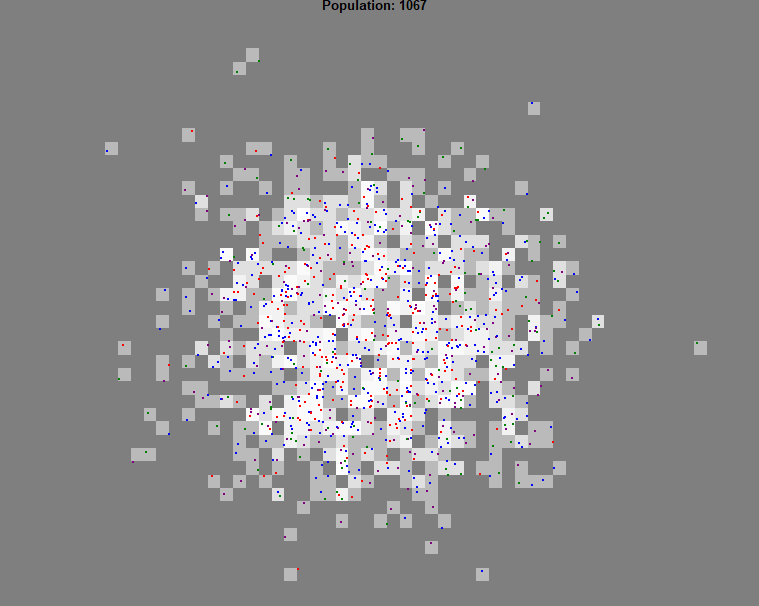
\includegraphics[scale = 0.8]{Graphics/city sim basic.png}
    \caption{Simulation of distribution of city consisting of household with basic psuedo-continuous utilities. Red, blue, purple, and green units represent income levels from lowest to highest respectively.\textsuperscript{\cite{pjcode}}}
    \label{fig:city sim}
\end{figure}






\end{document}